\documentclass[tikz,border=12pt]{standalone}
\usepackage[T1]{fontenc}
\usepackage{mathpazo}
\usepackage{amsmath,amssymb}
\usetikzlibrary{arrows.meta, positioning, calc, fit, decorations.pathreplacing}
\definecolor{stblue}{HTML}{7B97AD}
\definecolor{rwgold}{HTML}{B8995E}
\definecolor{sage}{HTML}{7A9A7E}
\definecolor{dkbrown}{HTML}{3D3530}
\definecolor{wmgray}{HTML}{7B7067}
\definecolor{cream}{HTML}{F9F6F0}
\definecolor{border}{HTML}{D4C9B8}
\definecolor{terracotta}{HTML}{C47A6A}
\definecolor{lavender}{HTML}{907EA0}

\begin{document}
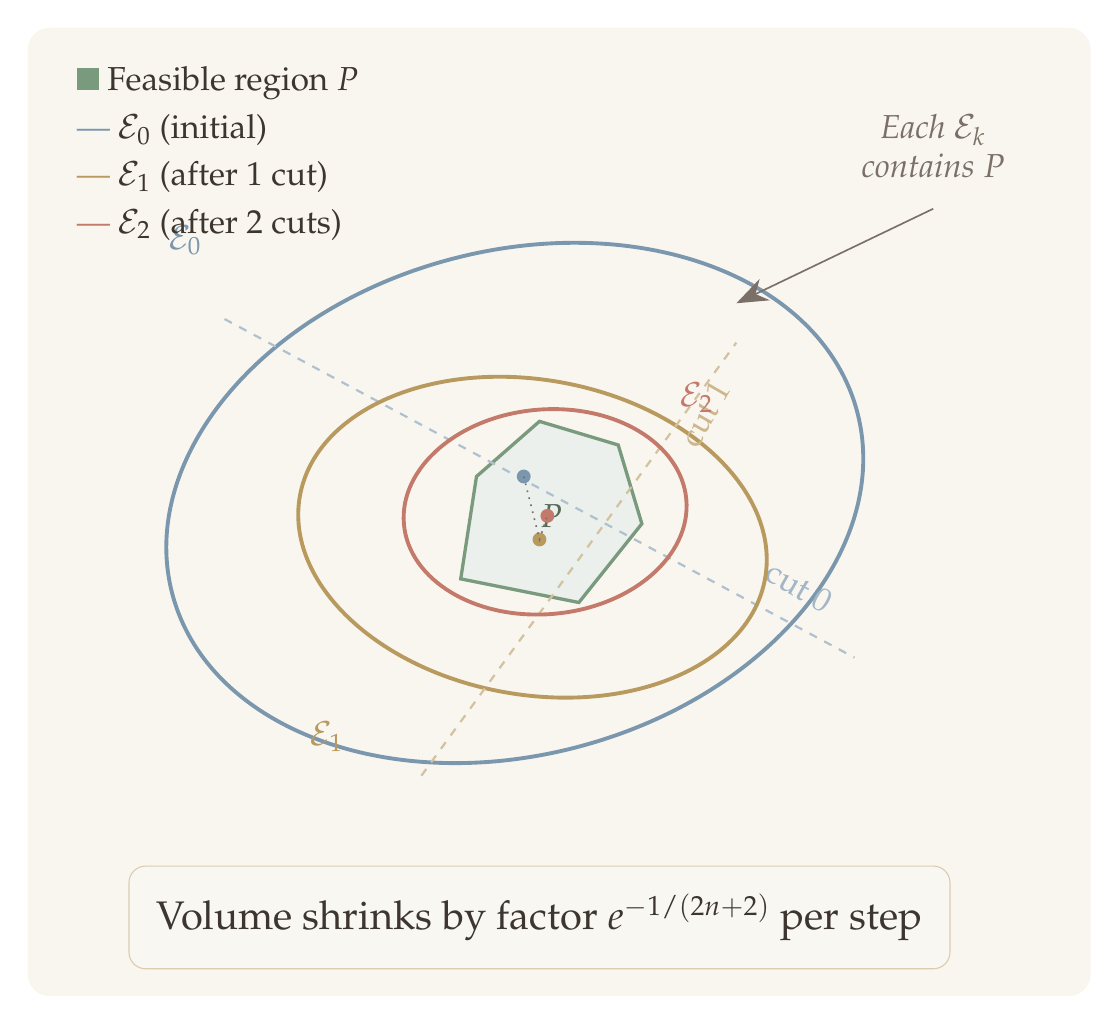
\begin{tikzpicture}[
    >={Stealth[length=4mm, width=3mm]},
    every node/.style={text=dkbrown},
  ]

  % Background
  \fill[cream, rounded corners=8pt] (-6.0,-5.8) rectangle (7.5,6.5);

  % === Feasible region (convex polygon) ===
  \fill[sage!15] (-0.5,-0.5) -- (1.0,-0.8) -- (1.8,0.2)
    -- (1.5,1.2) -- (0.5,1.5) -- (-0.3,0.8) -- cycle;
  \draw[sage, line width=1.2pt] (-0.5,-0.5) -- (1.0,-0.8) -- (1.8,0.2)
    -- (1.5,1.2) -- (0.5,1.5) -- (-0.3,0.8) -- cycle;
  \node[font=\large\bfseries, sage!70!black] at (0.65,0.3) {$P$};

  % === Ellipsoid E_0 (large, stblue) ===
  \draw[stblue, line width=1.4pt, rotate=15]
    (0.3,0.4) ellipse (4.5cm and 3.2cm);
  \node[font=\large\bfseries, stblue] at (-4.0,3.8) {$\mathcal{E}_0$};

  % Separating hyperplane 0 (dashed)
  \draw[stblue!60, line width=0.8pt, dashed]
    (-3.5, 2.8) -- (4.5, -1.5);
  \node[font=\large, stblue!70, rotate=-30] at (3.8, -0.6) {cut $0$};

  % === Ellipsoid E_1 (medium, rwgold) ===
  \draw[rwgold, line width=1.4pt, rotate=-10]
    (0.4, 0.1) ellipse (3.0cm and 2.0cm);
  \node[font=\large\bfseries, rwgold] at (-2.2, -2.5) {$\mathcal{E}_1$};

  % Separating hyperplane 1 (dashed)
  \draw[rwgold!60, line width=0.8pt, dashed]
    (-1.0, -3.0) -- (3.0, 2.5);
  \node[font=\large, rwgold!70, rotate=60] at (2.6, 1.6) {cut $1$};

  % === Ellipsoid E_2 (small, terracotta) ===
  \draw[terracotta, line width=1.4pt, rotate=5]
    (0.6, 0.3) ellipse (1.8cm and 1.3cm);
  \node[font=\large\bfseries, terracotta] at (2.5, 1.8) {$\mathcal{E}_2$};

  % Centers
  \fill[stblue] (0.3, 0.8) circle (2.5pt);
  \fill[rwgold] (0.5, 0.0) circle (2.5pt);
  \fill[terracotta] (0.6, 0.3) circle (2.5pt);

  % Path connecting centers
  \draw[wmgray, line width=0.6pt, dotted]
    (0.3,0.8) -- (0.5,0.0) -- (0.6,0.3);

  % Volume shrinkage annotation
  \node[font=\Large, text=dkbrown, align=center,
        fill=rwgold!8, draw=rwgold!50, rounded corners=6pt,
        inner sep=10pt] at (0.5, -4.8)
    {Volume shrinks by factor $e^{-1/(2n+2)}$ per step};

  % Legend
  \node[font=\large, anchor=west] at (-5.5, 5.8)
    {\textcolor{sage}{\rule{8pt}{8pt}} Feasible region $P$};
  \node[font=\large, anchor=west] at (-5.5, 5.2)
    {\textcolor{stblue}{---} $\mathcal{E}_0$ (initial)};
  \node[font=\large, anchor=west] at (-5.5, 4.6)
    {\textcolor{rwgold}{---} $\mathcal{E}_1$ (after 1 cut)};
  \node[font=\large, anchor=west] at (-5.5, 4.0)
    {\textcolor{terracotta}{---} $\mathcal{E}_2$ (after 2 cuts)};

  % Annotation: each ellipsoid contains P
  \node[font=\large\itshape, text=wmgray, align=center] at (5.5, 5.0)
    {Each $\mathcal{E}_k$\\contains $P$};
  \draw[->, wmgray, line width=0.6pt] (5.5, 4.2) -- (3.0, 3.0);

\end{tikzpicture}
\end{document}
